\section{Multi-Layer Perceptrons}

\subsection{Physiological Motivation}

\begin{frame}
  \frametitle{Physiological Motivation}
  
  \begin{center}
    \includegraphics[width=.7\linewidth]{\pngdir/neuron.\png}
  \end{center}
\end{frame}


%\begin{frame}
%  \frametitle{Physiological Motivation \cont}
%  
%  \structure{Synaptic transmission from a presynaptic neuron to a postsynaptic cell:}
%  
%  \begin{columns}
%    \column{.55\linewidth}
%      \begin{enumerate}
%        \item \structure{Action potential} traveling along the membrane of the presynaptic cell, until it reaches the synapse
%      \end{enumerate}
%%
%    \column{.4\linewidth}
%      \begin{center}
%        \includegraphics[width=\linewidth]{\jpgdir/synapse.\jpg}
%      \end{center}
%  \end{columns}
%\end{frame}
%
%
%\begin{frame}
%  \frametitle{Physiological Motivation \cont}
%  
%  \structure{Synaptic transmission from a presynaptic neuron to a postsynaptic cell:}
%  
%  \begin{columns}
%    \column{.55\linewidth}
%      \begin{enumerate}
%        \setcounter{enumi}{1}                 
%        \item \structure{Electrical depolarization} of the membrane at the synapse:
%        \begin{itemize}
%          \item Causes channels to open that are permeable to calcium ions
%          \item Calcium ions flow through the presynaptic membrane, rapidly increasing the calcium concentration in the interior.
%          \item Vesicles with neurotransmitter chemical open and dump their   content into synaptic cleft.
%        \end{itemize} 
%      \end{enumerate}
%%
%    \column{.4\linewidth}
%      \begin{center}
%        \includegraphics[width=\linewidth]{\jpgdir/synapse.\jpg}
%      \end{center}
%  \end{columns}
%\end{frame}
%
%
%\begin{frame}
%  \frametitle{Physiological Motivation \cont}
%  
%  \structure{Synaptic transmission from a presynaptic neuron to a postsynaptic cell:}
%  
%  \begin{columns}
%    \column{.55\linewidth}
%      \begin{enumerate}
%        \setcounter{enumi}{2}
%        \item \structure{Neurotransmitter} bind to chemical receptor molecules located on the membrane of the postsynaptic cell. \\[.2cm] \pause
%        \item Opening of ion channels in the postsynaptic cell membrane, causing ions to enter or exit the cell and change the local transmembrane potential: \structure{excitatory} or \structure{inhibitory postsynaptic potential (EPSP/IPSP)}.
%      \end{enumerate}
%%
%    \column{.4\linewidth}
%      \onslide<1->
%      \begin{center}
%        \includegraphics[width=\linewidth]{\jpgdir/synapse.\jpg}
%      \end{center}
%  \end{columns}
%\end{frame}
%
%
%\begin{frame}
%  \frametitle{Physiological Motivation \cont}
%  
%  \structure{Synaptic transmission from a presynaptic neuron to a postsynaptic cell:}
%  
%  \begin{columns}
%    \column{.55\linewidth}
%      \begin{enumerate}
%        \setcounter{enumi}{4}
%        \item Due to thermal shaking, neurotransmitter molecules eventually break loose from the receptors and drift away. \\[.2cm] \pause
%        \item The neurotransmitter is either reabsorbed by the presynaptic cell, and then repackaged for future release, or else it is broken down metabolically.
%      \end{enumerate}
%%
%    \column{.4\linewidth}
%      \onslide<1->
%      \begin{center}
%        \includegraphics[width=\linewidth]{\jpgdir/synapse.\jpg}
%      \end{center}
%  \end{columns}
%\end{frame}
%
%
%\begin{frame}
%  \frametitle{Physiological Motivation \cont}
%  
%  \structure{Creating new action potentials} \\[.25cm]
%
%  \begin{itemize}
%    \item EPSPs resulting from transmitter release at a single synapse are generally far too small to trigger a spike in the postsynaptic neuron. \\[.15cm]
%    \item A neuron may receive inputs from thousands of other neurons. \\[.15cm]
%    \item If the postsynaptic cell is sufficiently depolarized, an \structure{action potential} will occur. \\[.15cm]
%    \item Action potentials are not graded; they are all-or-none responses.
%  \end{itemize}
%\end{frame}
%
%
%\begin{frame}
%  \frametitle{Physiological Motivation \cont}
%  
%  \structure{Creating new action potentials} \\[.25cm]
%
%  \begin{itemize}
%    \item Postsynaptic potentials are subject to summation:
%    \begin{itemize}
%      \item Spatial summation
%      \item Temporal summation
%    \end{itemize}
%  \end{itemize}
%
%  \begin{center}
%    \includegraphics[width=.6\linewidth]{\jpgdir/EPSP_summation.\jpg}
%  \end{center}
%\end{frame}


\subsection{Topology and Activation Functions}

\begin{frame}
  \frametitle{Multi-Layer Perceptrons}

  \structure{Topology}

  \begin{center}
    \resizebox{.8\linewidth}{!}{
      \input{\texfigdir/mlp.pstex_t}
    }
  \end{center}
\end{frame}


\begin{frame}
  \frametitle{Multi-Layer Perceptrons \cont}

  \structure{Activation Functions}

  \begin{center}
    \resizebox{.8\linewidth}{!}{
      \input{\texfigdir/activation.pstex_t}
    }
  \end{center}

  \begin{displaymath}
    \text{net}_j^{(l)} = \sum_{i=1}^{M^{(l-1)}} y_i^{(l-1)} w_{ij}^{(l)} - w_{0j}^{(l)}
  \end{displaymath}

  \begin{displaymath}
    y_j^{(l)} = f(\text{net}_j^{(l)})
  \end{displaymath}
\end{frame}


\subsection{Backpropagation Algorithm}

\begin{frame}
  \frametitle{Backpropagation Algorithm}

  \structure{Supervised Learning Algorithm}

  \begin{itemize}
    \item Gradient descent to adjust the weights reducing the training error $\varepsilon$:
      \begin{displaymath}
        \Delta w_{ij}^{(l)} = - \eta \, \frac{\partial \varepsilon}{\partial w_{ij}^{(l)}}
      \end{displaymath}

    \item Typical error function: \structure{mean squared error}
      \begin{displaymath}
        \varepsilon_{MSE}(\vec{w}) = \frac{1}{2} \sum_{k=1}^{M^{(L)}} (t_k - y_k^{(L)})^2
      \end{displaymath}
  \end{itemize}
\end{frame}


\newcommand{\err}{\varepsilon_{\text{MSE}}}
\newcommand{\net}[2]{\text{net}_{#1}^{(#2)}}
\newcommand{\w}[2]{w_{#1}^{(#2)}}
\newcommand{\y}[2]{y_{#1}^{(#2)}}

\begin{frame}
  \frametitle{Backpropagation Algorithm \cont}

  \structure{Adjusting the weights $\w{jk}{L}$ of the output layer}

  \begin{columns}
    \column{.7\linewidth}
      {\footnotesize
      \begin{displaymath}
        \frac{\partial \err}{\partial \w{jk}{L}} =
        \frac{\partial \err}{\partial \net{k}{L}} \cdot \frac{\partial \net{k}{L}}{\partial \w{jk}{L}} =
        - \delta_k^{(L)} \cdot y_j^{(L-1)}
      \end{displaymath}
      }
      \vspace*{.5cm}

      \hspace*{0.4cm}\structure{The \emph{sensitivity} $\delta_k^{(L)}$:}

      {\footnotesize
      \begin{eqnarray*}
        \delta_k^{(L)} 
        & = & - \frac{\partial \err}{\partial \net{k}{L}}
          =   - \frac{\partial \err}{\partial \y{k}{L}} \cdot \frac{\partial \y{k}{L}}{\partial \net{k}{L}} \\
        & = & (t_k - \y{k}{L}) \, f'(\net{k}{L})
      \end{eqnarray*}
      }
    \column{.3\linewidth}
      \begin{center}
        \resizebox{\linewidth}{!}{
          \input{\texfigdir/backpropagation3.pstex_t}
        }
      \end{center}
  \end{columns}
\end{frame}


\begin{frame}
  \frametitle{Backpropagation Algorithm \cont}

  \structure{Adjusting the weights $\w{jk}{l}$ of the hidden layers} \\[.25cm]

  \begin{itemize}
    \item Desired output values for the hidden layers are not known. \\[.15cm]
    \item For the weights $\w{ij}{L-1}$ of the last hidden layer:
  \end{itemize}

  \begin{columns}
    \column{.6\linewidth}
      \footnotesize
      \vspace*{0.5cm}
      \begin{eqnarray*}
        \frac{\partial \err}{\partial \w{ij}{L-1}} & = &
        \frac{\partial \err}{\partial \y{j}{L-1}} \cdot
        \frac{\partial \y{j}{L-1}}{\partial \net{j}{L-1}} \cdot
        \frac{\partial \net{j}{L-1}}{\partial \w{ij}{L-1}} \\
        & = & \frac{\partial \err}{\partial \y{j}{L-1}} \cdot
        f'(\net{j}{L-1}) \cdot \y{i}{L-2}
      \end{eqnarray*}
    \column{.4\linewidth}
      \begin{center}
        \resizebox{.9\linewidth}{!}{
          \input{\texfigdir/backpropagation2.pstex_t}
        }
      \end{center}
  \end{columns}
\end{frame}


\begin{frame}
  \frametitle{Backpropagation Algorithm \cont}
%
   \begin{itemize}
      \vspace*{-0.5cm}
     \item {\small The differentiation of $\partial \err$ w.\,r.\,t.\ $\y{j}{L-1}$ can be computed as the sum of the sensitivity values $\delta_k^{(L)}$ of the layer above weighted by the weights $\w{jk}{L}$:}
   \end{itemize}
  \begin{columns}
    \column{.6\linewidth}
      \footnotesize
       \vspace*{-0.5cm}
      \begin{eqnarray*}
        \frac{\partial \err}{\partial \y{j}{L-1}} & = &
        \frac{\partial}{\partial \y{j}{L-1}} \Bigg[
          \frac{1}{2} \sum_{k=1}^{M^{(L)}} (t_k - \y{k}{L})^2      
          \Bigg] \\ 
        & = & - \sum_{k=1}^{M^{(L)}} (t_k - \y{k}{L}) \, \frac{\partial\y{k}{L}}{\partial\y{j}{L-1}} \\
        & = & - \sum_{k=1}^{M^{(L)}} (t_k - \y{k}{L}) \, \frac{\partial\y{k}{L}}{\partial\net{k}{L}} \cdot
                \frac{\partial\net{k}{L}}{\partial\y{j}{L-1}} \nonumber \\
        & = & - \sum_{k=1}^{M^{(L)}} (t_k - \y{k}{L}) \, f'(\net{k}{L}) \, \w{jk}{L} \\
        & = & - \sum_{k=1}^{M^{(L)}} \delta_k^{(L)} \w{jk}{L}
      \end{eqnarray*}
    \column{.4\linewidth}
      \begin{center}
        \resizebox{.8\linewidth}{!}{
          \input{\texfigdir/backpropagation.pstex_t}
        }
      \end{center}
  \end{columns}
\end{frame}


\begin{frame}
  \frametitle{Backpropagation Algorithm \cont}

  \structure{Sensivity $\delta_j^{(l)}$ for any hidden layer $l$, $0<l<L$}

  \begin{displaymath}
    \delta_j^{(l)} = f'(\net{j}{l}) \, \sum_{k=1}^{M^{(l+1)}} \w{jk}{l+1} \, \delta_k^{(l+1)}
  \end{displaymath}
  \pspread

  \structure{Update rule}

  \begin{displaymath}
    \Delta\w{ij}{l} = \eta \, \delta_j^{(l)} \, \y{i}{l-1}
  \end{displaymath} 
\end{frame}

\begin{frame}{Linear Network in Matrix Notation}
	\begin{itemize}
		\item Fully connected layers can be expressed as matrix multiplications.
		\begin{align*}
		\hat{\mat y}= \hat{\mat f}_{3}(\hat{\mat f}_{2}(\hat{\mat f}_{1}(\mat x)))) = \mat W_3 \mat W_2 \mat W_1\mat x
		\end{align*}
		\onslide<2->{ \item Associated loss function:
			\begin{align*}
			L(\mat \theta)= \frac{1}{2} || \mat W_3 \mat W_2  \mat W_1 \mat x - \mat y ||_2^2 
			\end{align*}}
		\onslide<3->{\item Gradients?}
	\end{itemize}
\end{frame}

\begin{frame}{Linear Network in Matrix notation}
	\begin{center}
		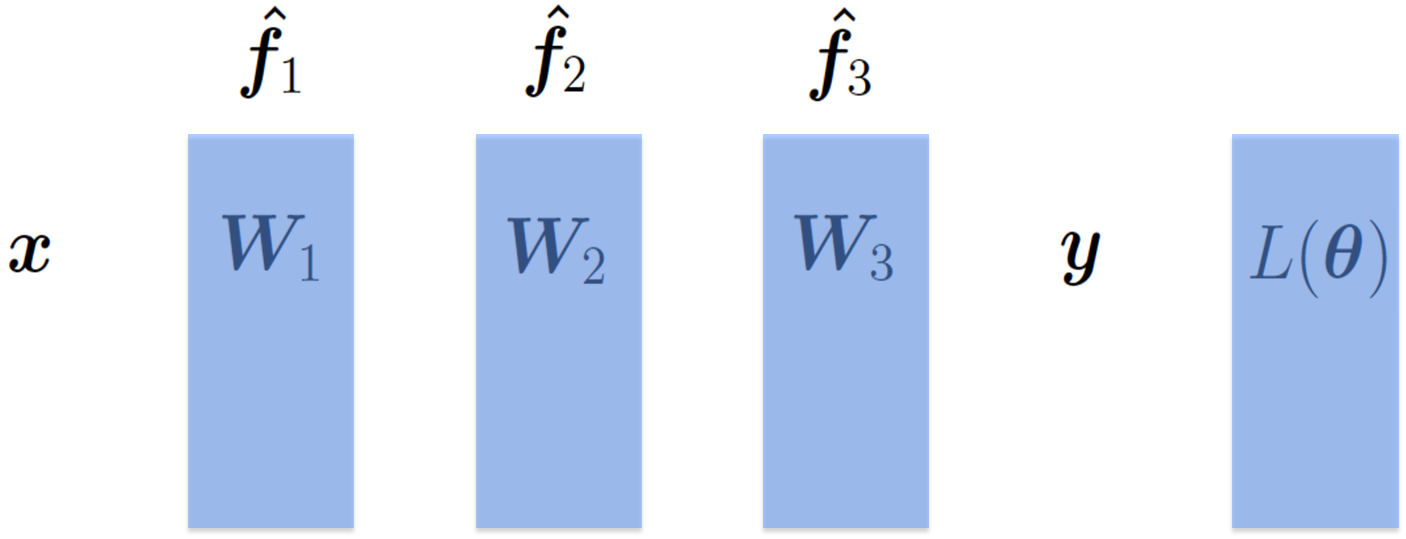
\includegraphics[width=0.797\textwidth]{png/gradient_derviation1.png}
	\end{center}
\end{frame}

\begin{frame}{Linear Network in Matrix notation}
	\begin{center}
		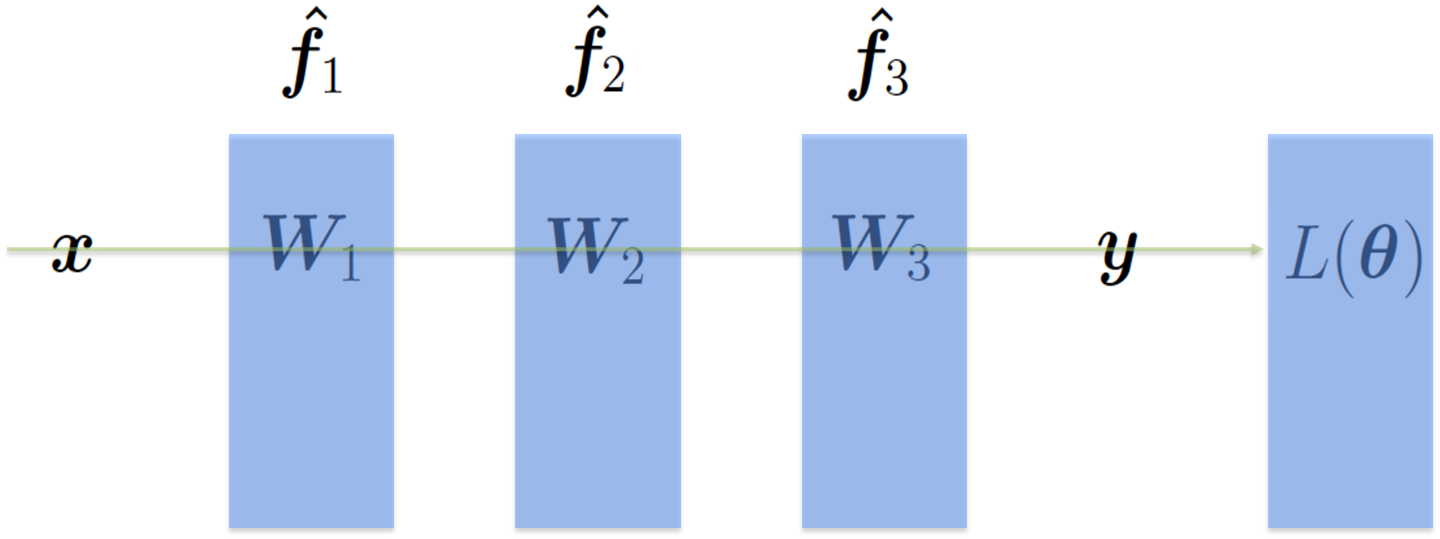
\includegraphics[width=0.8\textwidth]{png/gradient_derviation2.png}
	\end{center}
\end{frame}

\begin{frame}{Linear Network in Matrix notation}
	\begin{center}
		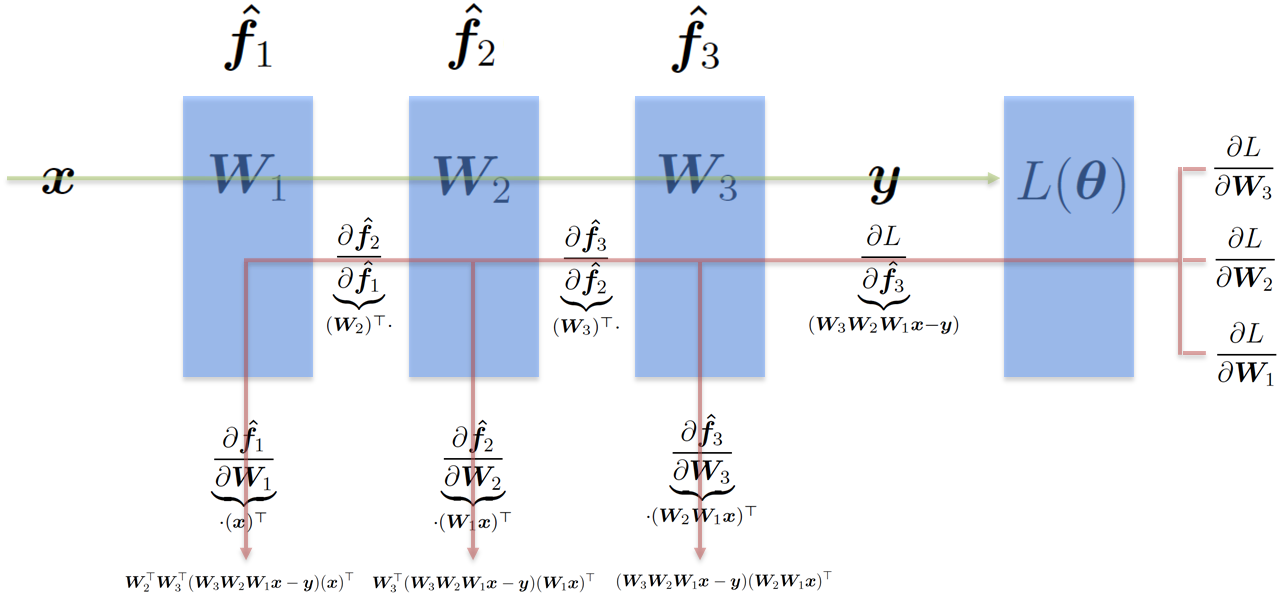
\includegraphics[width=0.9\textwidth]{png/gradient_derviation3.png}
	\end{center}
\end{frame}

\subsection{Lessons Learned}

\begin{frame}
  \frametitle{Lessons Learned}
  
  \begin{itemize}  
    \item Physiological background: neurons, synapses, action potentials, \\[.25cm]
    \item Topology of multi-layer perceptrons \\[.25cm]
    \item Activation functions \\[.25cm]
    \item Backpropagation algorithm: gradient descent method
  \end{itemize}
\end{frame}

{
\usebackgroundtemplate{\includegraphics[width=\paperwidth]{png/nextTime.png}}
\begin{frame}[plain]
\end{frame}
}


\subsection{Further Readings}

\begin{frame}
  \frametitle{Further Readings}
  
  \structure{\ldots from physiology:}\\[.25cm]
  
  \begin{itemize}
    \item Robert F.\ Schmidt (Hrsg.): \\
      \structure{Neuro- und Sinnesphysiologie}, \\
      3., korrigierte Auflage, Springer, Berlin, 1998 \\[.25cm]
    \item Robert F.\ Schmidt, Florian Lang, Martin Heckmann (Hrsg.): \\
      \structure{Physiologie des Menschen mit Pathophysiologie}, \\
      31., neu bearb. u. aktual. Auflage, Springer, Berlin, 2010
  \end{itemize}
\end{frame}
